\casesection{B\'elanger surface profile\label{case:belanger}}


\paragraph*{Purpose}
The purpose of this validation case is to examine the performance of \DFLOWFM for a schematized channel flow simulation. For stationary flow through a river with a rectangular cross-section, the B\'elanger surface profile equation can be utilized to compare the numerical solution with.


\paragraph*{Linked claims}
Claims that are related to the current test case are:
\begin{itemize}
\item \clrefnoh{cl:generalGrids}
\end{itemize}


\paragraph*{Approach}
A straight channel with a rectangular cross-section is defined. Given an inflow discharge $Q$, a channel width $B$, a bottom slope $i_b$ and a Ch\'ezy friction factor $C$, the distance between the free surface profile and the bed profile can be described by the B\'elanger equation for $d$ as the water depth:
\begin{equation}
\frac{\mathrm{d}d}{\mathrm{d}x} = i_b \frac{d^3 - d_e^3}{d^3 - d_g^3}
\end{equation}
with $d_e$ the equilibrium depth and $d_g$ the limit depth (associated with $\mathrm{Fr} = 1$) following:
\begin{equation}
d_e = \left(\frac{Q^2}{B^2 g}\right)^{1/3} \hspace{1cm} \textrm{and} \hspace{1cm} d_g = \left(\frac{Q^2}{B^2 C^2 i_b}  \right)^{1/3}.
\end{equation}
Given a certain inflow discharge $Q_{in}$ and a certain outflow water level condition $h_{out}$, the surface profile can hence numerically be estimated in the most simple way as:
\begin{equation}
\frac{d_{i} - d_{i-1}}{\Delta x} = i_b \frac{d^3_{i} - d_e^3}{d^3_{i} - d_g^3},
\end{equation}
having $d_i = h_{out} + i_b L$ at the outflow boundary. This, in fact \emph{semi-analytical}, solution can be used for comparison.
%\todo{Belanger curve schaalt met $i\_b$, dat betekent dat er geen backwater is als er geen bodemhelling is. Formule klopt niet voor vlakke bodems}


\paragraph*{Model description}
For this test case, one single computational grid is generated. The computational domain has the sizes $L \times B = 100$ km $\times$ $20$ m. The grid counts $200 \times 1$ cells. The cell size is $500 \times 20$ m$^2$ everywhere. The bed slope $i_b$ is $10^{-4}$. The inflow discharge is $Q = 600$ m$^3$/s. The Ch\'ezy coefficient is $C = 65$ m$^{1/2}$/s. The outflow water \emph{level} is set equal to 0 m (w.r.t.\ reference), i.e.\ the water \emph{depth} is hence equal to 10 meters.

Recall that the water depth is computed as the difference between the upstream water level (computed at the \emph{cell center}) and the bed level at the velocity point (computed at the \emph{cell face}), invoking a $\Delta x/2$ spatial shift. In the computational model, the bed level at the outflow boundary is equal to -10~m+NAP, whereas a water level equal to 0~m+NAP is imposed at the outflow boundary. Since the location for the water level outflow boundary condition is also $\Delta x/2$ outside the grid (mirrored location), the water level boundary conditions yields a bed level equal to $b|_{x = L + \Delta x} = -i_b \cdot (L + \Delta x) = -10^{-4}\cdot 100500 = -10.05$~m (given a zero bed level at the entrance of the channel). Hence, the outflow water depth equals $d_{out} = h_{out} - b_{out} = 0 - (-10.05) = 10.05$~m, at $x = L + \Delta x$.




\paragraph*{Results}
The result from \DFLOWFM for the water \emph{depth} is shown in \Fref{fig:belangersingledepth} in combination with its semi-analytical equivalent. The semi-analytical solution is based on the equation for the B\'elanger surface profile.

\begin{figure}[h!]
\begin{center}
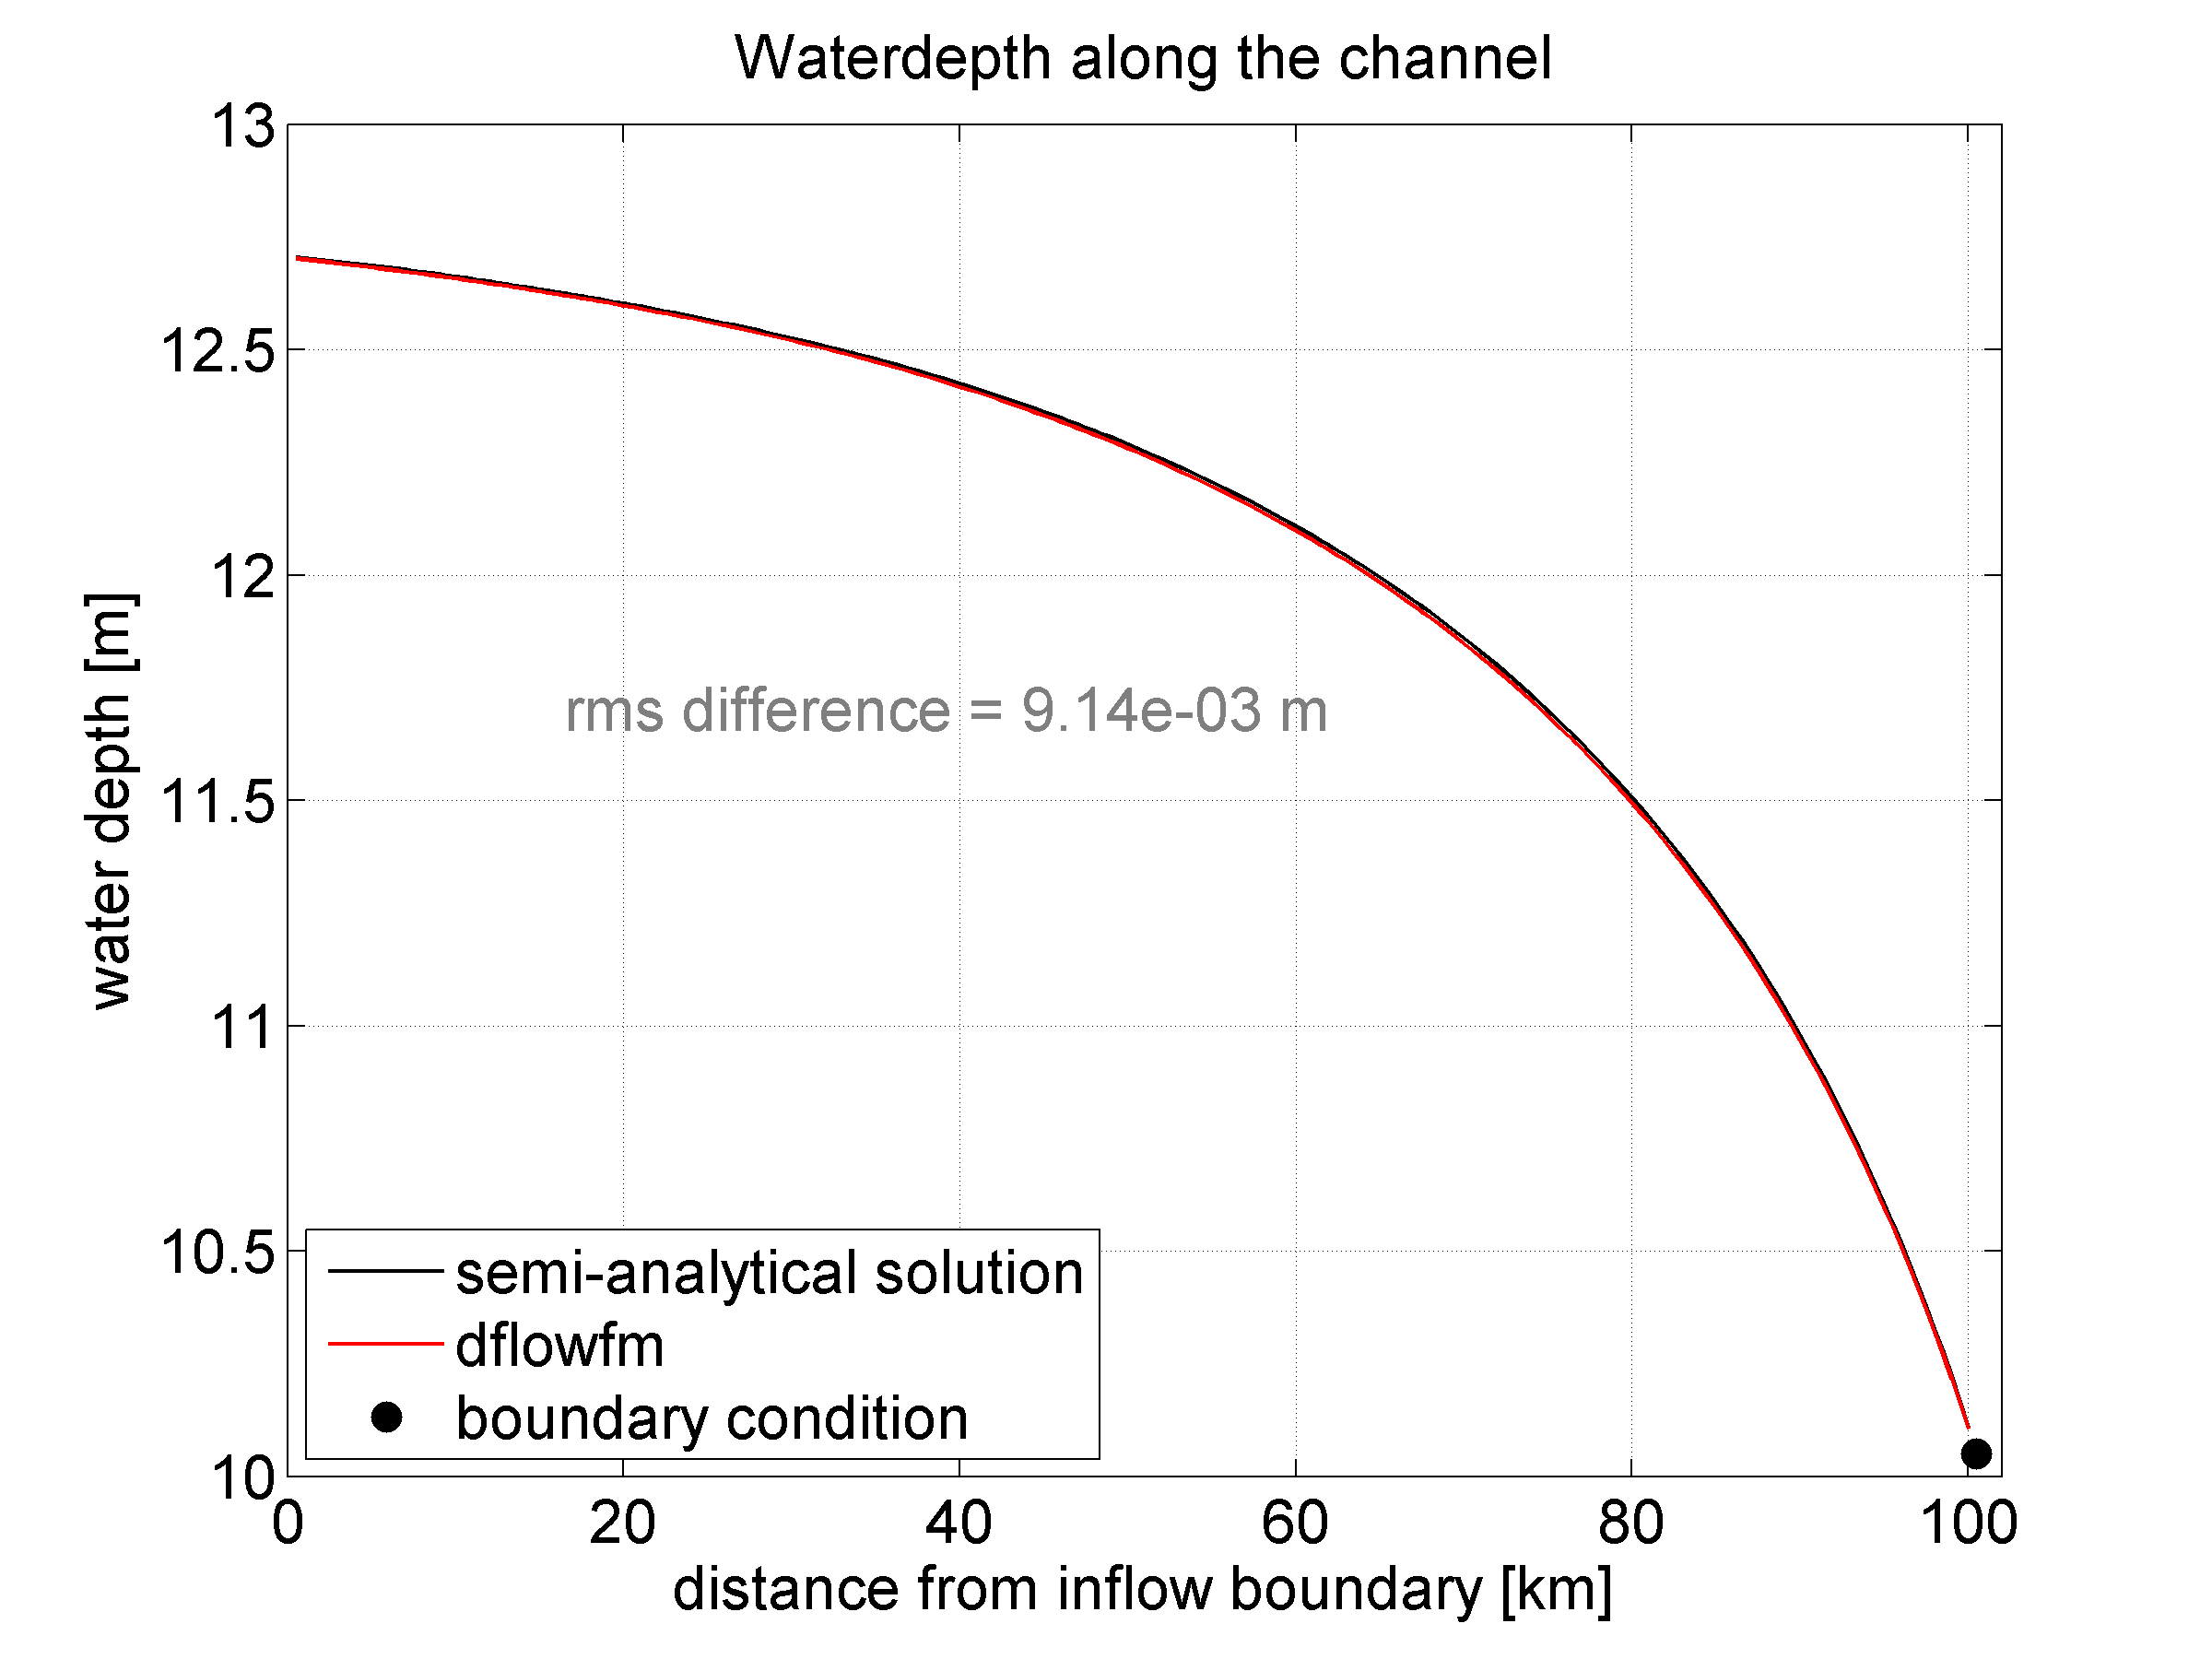
\includegraphics[width=0.8\columnwidth]{figures/waterdepth.png}
\end{center}\caption{Comparison of the numerical solution and the semi-analytical solution for the water depth. \label{fig:belangersingledepth}}
\end{figure}

The root-mean-square difference between the numerical outcome from \DFLOWFM and the semi-analytical solution is shown in \Fref{fig:belangersingledepth} as well. This rms-difference is of the order of $10^{-3}$ m. 


\paragraph*{Conclusion}
For the B\'elanger test case under consideration, the numerical solution approaches the semi-analytical solution up to an overall root-mean-square difference of the order of $10^{-3}$ m.




\paragraph*{Version}
This test has been carried out with version dflow-fm-x64-1.1.116.36629.


